\chapter{A Comprehensive Look at RAII}

Resource management is probably the second most frequent thing a program does, after computing. But just because it's frequently done does not mean it's visible---some languages hide most, or all, resource management from the user. And just because it is hidden, does not mean it's not there.

Every program needs to use some memory, and memory is a resource. A program would be of no use if it never interacted with the outside world in some way, at least to print the result, and input and output channels (files, sockets, and so on) are resources.

In this chapter, we will start by answering the following questions:

\begin{itemize}
\item
  What is considered a resource in a C++ program?
\item
  What are the key concerns for managing resources in C++?
\end{itemize}

Then, we will introduce \textbf{Resource Acquisition is Initialization} (\textbf{RAII}) and explain how it helps in efficient resource management in C++ by answering these questions:

\begin{itemize}
\item
  What is the standard approach for managing resources in C++ (RAII)?
\item
  How does RAII solve the problems of resource management?
\end{itemize}

We will end the chapter with a discussion about the implications and possible concerns of using RAII by providing the answers to these questions:

\begin{itemize}
\item
  What are the precautions that must be taken when writing RAII objects?
\item
  What are the consequences of using RAII for resource management?
\end{itemize}

C++, with its zero-overhead abstraction philosophy, does not hide resources or their management at the core language level. But we would do well to not confuse hiding resources with managing them.

\section{Technical requirements}

Here are some useful links:

\begin{itemize}
\item
  Google Test unit testing framework: https://github.com/google/googletest
\item
  Google Benchmark library: https://github.com/google/benchmark
\item
  Example code: https://github.com/PacktPublishing/Hands-On-Design-Patterns-with-CPP-Second-Edition/tree/master/Chapter05{}{}
\end{itemize}

\section{Resource management in C++}

Every program operates on resources and needs to manage them. The most commonly used resource is memory, of course. Hence, you often read about \textbf{memory} \textbf{management} in C++. But really, resources can be just about anything. Many programs exist specifically to manage real, tangible physical resources, or the more ephemeral (but no less valuable) digital ones. Money in bank accounts, airline seats, car parts and assembled cars, or even crates of milk---in today's world, if it is something that needs to be counted and tracked, there is a piece of software somewhere that is doing it. But even in a program that does pure computations, there may be varied and complex resources, unless the program also eschews abstractions and operates at the level of bare numbers. For example, a physics simulation program may have particles as resources.

All of these resources have one thing in common---they need to be accounted for. They should not vanish without a trace, and a program should not just make up resources that don't really exist. Often, a specific instance of a resource is needed---you would not want someone else's purchase to be debited from your bank account; the specific instance of the resource matters. Thus, the most important consideration when evaluating different approaches to resource management is correctness---how well does the design ensure that resources are managed properly, how easy is it to make a mistake, and how hard would it be to find such a mistake? It should come as no surprise, then, that we use a testing framework to present the coding examples of resource management in this chapter.

\subsection{Installing the microbenchmark library}

In our case, we are interested in the efficiency of memory allocations and small fragments of code that may contain such allocations. The appropriate tool for measuring the performance of small fragments of code is a microbenchmark. There are many microbenchmark libraries and tools out there; in this book, we will use the Google Benchmark library. To follow along with the examples in this chapter, you must first download and install the library (follow the instructions in the \texttt{Readme.md} file). Then you can compile and run the examples. You can build the sample files included with the library to see how to build a benchmark on your particular system; you can also use the example benchmark from this chapter's repository:

\begin{code}
// Example 01
#include <stdlib.h>
#include "benchmark/benchmark.h"
void BM_malloc(benchmark::State& state) {
  constexpr size_t size = 1024;
  for (auto _ : state) {
    void* p = malloc(size);
    benchmark::DoNotOptimize(p);
    free(p);
  }
  state.SetItemsProcessed(state.iterations());
}
BENCHMARK(BM_malloc);
BENCHMARK_MAIN();
\end{code}

Note the call to \texttt{DoNotOptimize()}: it's a special function that doesn't generate any code but tricks the compiler into thinking that its argument is necessary and cannot be optimized away. Without this, the compiler will probably figure out that the entire benchmark loop has no observable effect and can be optimized to nothing.

On a Linux machine, the command to build and run a benchmark program called \texttt{01\_benchmark.C} might look something like this:

\begin{code}
$CXX 01_benchmark.C -I. -I$GBENCH_DIR/include 鈥揙3 \
  --std=c++17 $GBENCH_DIR/lib/libbenchmark.a -lpthread \
  -o 01_benchmark && ./01_benchmark
\end{code}

Here, \texttt{\$CXX} is your C++ compiler, such as \texttt{g++} or \texttt{clang++}, and \texttt{\$GBENCH\_DIR} is the directory where the benchmark is installed.

The preceding example should print something like this:

\pandocbounded{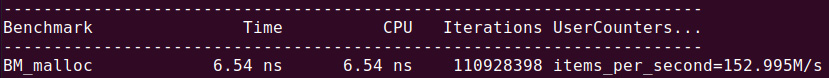
\includegraphics[keepaspectratio]{./image/Figure_5.1_B19262.jpg}}

On this particular machine, a single iteration (one pair of calls to \texttt{malloc()} and \texttt{free()}) takes 6.37 nanoseconds, which translates into 157 million memory allocations per second.

Sometimes we have to benchmark very short operations:

\begin{code}
void BM_increment(benchmark::State& state) {
  size_t i = 0;
  for (auto _ : state) {
    ++i;
    benchmark::DoNotOptimize(i);
  }
  state.SetItemsProcessed(state.iterations());
}
\end{code}

We may be reasonably concerned about the overhead of the benchmark loop itself. In such cases, we can execute multiple copies of the benchmarked operation within the body of the loop. We can even get the C++ preprocessor to make copies for us:

\begin{code}
// Example 02
#define REPEAT2(x) x x
#define REPEAT4(x) REPEAT2(x) REPEAT2(x)
#define REPEAT8(x) REPEAT4(x) REPEAT4(x)
#define REPEAT16(x) REPEAT8(x) REPEAT8(x)
#define REPEAT32(x) REPEAT16(x) REPEAT16(x)
#define REPEAT(x) REPEAT32(x)
void BM_increment32(benchmark::State& state) {
  size_t i = 0;
  for (auto _ : state) {
    REPEAT(
      ++i;
      benchmark::DoNotOptimize(i);
    )
  }
  state.SetItemsProcessed(32*state.iterations());
}
\end{code}

The time of a ``\emph{single}'' iteration now includes 32 iterations, so it is much easier to use the items per second value. Remember to include repeat count in the number of items processed:

\pandocbounded{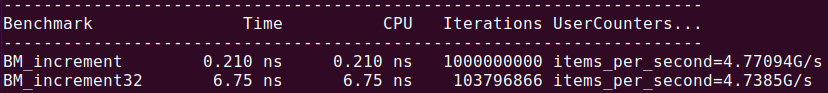
\includegraphics[keepaspectratio]{./image/Figure_5.2_B19262.jpg}}

Writing fast programs is all well and good, but they have to be correct first. To that end, we need to write tests, so we also need a testing framework.

\subsection{Installing Google Test}

We will be testing very small fragments of code for correctness. On the one hand, this is simply because each fragment illustrates a specific concept or idea. On the other hand, even in a large-scale software system, resource management is done by small building blocks of code. They may combine to form a quite complex resource manager, but each block performs a specific function and is testable. The appropriate testing system for this situation is a unit testing framework. There are many such frameworks to choose from; in this book, we will use the Google Test unit testing framework. To follow along with the examples in this chapter, you must first download and install the framework (follow the instructions in the \texttt{README} file). Once installed, you can compile and run the examples. You can build the sample tests included with the library to see how to build and link with Google Test on your particular system; you can also use the example from this chapter's repository:

\begin{code}
#include <vector>
#include "gtest/gtest.h"
TEST(Memory, Vector) {
  std::vector<int> v(10);
  EXPECT_EQ(10u, v.size());
  EXPECT_LE(10u, v.capacity());
}
\end{code}

On a Linux machine, the command to build and run a \texttt{02\_test.C} test might look something like this:

\begin{code}
$CXX 02_test.C -I. -I$GTEST_DIR/include -g -O0 -I. \
  -Wall -Wextra -Werror -pedantic --std=c++17 \
  $GTEST_DIR/lib/libgtest.a $GTEST_DIR/lib/libgtest_main.a\
  -lpthread -lrt -lm -o -2_test && ./02_test
\end{code}

Here, \texttt{\$CXX} is your C++ compiler, such as \texttt{g++} or \texttt{clang++}, and \texttt{\$GTEST\_DIR} is the directory where Google Test is installed. If all tests pass, you should get this output:

\begin{code}
Running main() from gtest_main.cc
[==========] Running 1 test from 1 test case.
[----------] Global test environment set-up.
[----------] 1 test from Memory
[ RUN      ] Memory.Vector
[       OK ] Memory.Vector (0 ms)
[----------] 1 test from Memory (0 ms total)
[----------] Global test environment tear-down
[==========] 1 test from 1 test case ran. (0 ms total)
[  PASSED  ] 1 test.
\end{code}

Writing good tests is an art. We have to identify the aspects of our code that need to be validated and come up with ways to observe these aspects. In this chapter, we are interested in resource management, so let us see how we can test the utilization and release of resources.

\subsection{Counting resources}

A unit testing framework, such as Google Test, allows us to execute some code and verify that the results are what they should be. The results that we can look at include any variable or expression that we can access from the test program. That definition does not extend, for example, to the amount of memory that is currently in use. So, if we want to verify that resources are not disappearing, we have to count them.

In the following simple test fixture, we use a special resource class instead of, say, the \texttt{int} keyword. This class is instrumented to count how many objects of this type have been created, and how many are currently alive:

\begin{code}
// Example 03
struct object_counter {
  static int count;
  static int all_count;
  object_counter() { ++count; ++all_count; }
  ~object_counter() { --count; }
};
int object_counter::count = 0;
int object_counter::all_count = 0;
\end{code}

Now we can test that our program manages resources correctly, as follows:

\begin{code}
// Example 03
#include "gtest/gtest.h"
TEST(Memory, NewDelete) {
  object_counter::all_count = object_counter::count = 0;
  object_counter* p = new object_counter;
  EXPECT_EQ(1, object_counter::count);
  EXPECT_EQ(1, object_counter::all_count);
  delete p;
  EXPECT_EQ(0, object_counter::count);
  EXPECT_EQ(1, object_counter::all_count);
}
\end{code}

In Google Test, every test is implemented as a \textbf{test fixture}. There are several types; the simplest one is a standalone test function, such as the one we use here. Running this simple test program tells us that the test has passed, as follows:

\begin{code}
[----------] 1 test from Memory
[ RUN      ] Memory.NewDelete
[       OK ] Memory.NewDelete (0 ms)
[----------] 1 test from Memory (0 ms total)
[  PASSED  ] 1 test.
\end{code}

The expected results are verified using one of the \texttt{EXPECT\_*} macros and any test failures will be reported. This test verifies that, after creating and deleting an instance of the type \texttt{object\_counter}, there are no such objects left, and that exactly one was constructed.

\section{Dangers of manual resource management}

C++ allows us to manage resources almost at the hardware level, and someone, somewhere, must indeed manage them at this level. The latter is actually true for every language, even the high-level ones that do not expose such details to the programmers. But \emph{somewhere} does not have to be in your program! Before we learn the C++ solutions and tools for resource management, let's first understand the problems that arise from not using any such tools.

\subsection{Manual resource management is error-prone}

The first and most obvious danger of managing every resource manually, with explicit calls to acquire and release each one, is that it is easy to forget the latter. For example, see the following:

\begin{code}
{
  object_counter* p = new object_counter;
  ... many more lines of code ...
  // Were we supposed to do something here?
  // Can't remember now...
}
\end{code}

We are now leaking a resource (the \texttt{object\_counter} objects, in this case). If we did this in a unit test, it would fail, as follows:

\begin{code}
// Example 04
TEST(Memory, Leak1) {
  object_counter::all_count = object_counter::count = 0;
  object_counter* p = new object_counter;
  EXPECT_EQ(1, object_counter::count);
  EXPECT_EQ(1, object_counter::all_count);
  //delete p;  // Forgot that
  EXPECT_EQ(0, object_counter::count); // This test fails!
  EXPECT_EQ(1, object_counter::all_count);
}
\end{code}

You can see the failing tests, and the location of the failures, as reported by the unit test framework:

\begin{code}
[ RUN      ] Memory.Leak1
04_memory.C:31: Failure
Expected equality of these values:
  0
  object_counter::count
    Which is: 1
[  FAILED  ] Memory.Leak1 (0 ms)
\end{code}

In a real program, finding such errors is much harder. Memory debuggers and sanitizers can help with memory leaks, but they require that the program actually execute the buggy code, so they depend on the test coverage.

The resource leaks can be much subtler and harder to find, too. Consider this code, where we did not forget to release the resource:

\begin{code}
bool process(... some parameters ... ) {
  object_counter* p = new object_counter;
  ... many more lines of code ...
  delete p;    // A-ha, we remembered!
  return true;    // Success
}
\end{code}

During subsequent maintenance, a possible failure condition was discovered, and the appropriate test was added:

\begin{code}
bool process(... some parameters ... ) {
  object_counter* p = new object_counter;
  ... many more lines of code ...
  if (!success) return false;   // Failure, cannot continue
  ... even more lines of code ...
  delete p;    // Still here
  return true;    // Success
}
\end{code}

This change introduced a subtle bug---now, resources are leaked only if the intermediate computation has failed and triggered the early return. If the failure is rare enough, this mistake may escape all tests, even if the testing process employs regular memory sanitizer runs. This mistake is also all too easy to make since the edit could be made in a place far removed from both the construction and deletion of the object, and nothing in the immediate context gives the programmer a hint that a resource needs to be released.

The alternative to leaking a resource, in this case, is to release it. Note that this leads to some code duplication:

\begin{code}
bool process(... some parameters ... ) {
  object_counter* p = new object_counter;
  ... many more lines of code ...
  if (!success) {
    delete p;
    return false;    // Failure, cannot continue
  }
  ... even more lines of code ...
  delete p;    // Still here
  return true;    // Success
}
\end{code}

As with any code duplication, there comes the danger of code divergence. Let's say that the next round of code enhancements required more than one \texttt{object\_counter}, and an array of them is now allocated as follows:

\begin{code}
bool process(... some parameters ... ) {
  object_counter* p = new object_counter[10]; // Array now
  ... many more lines of code ...
  if (!success) {
    delete p;
    return false;     // Old scalar delete
  }
  ... even more lines of code ...
  delete [] p;    // Matching array delete
  return true;    // Success
}
\end{code}

If we change \texttt{new} to the \texttt{new} array, we must change \texttt{delete} as well; the thought goes, there is probably one at the end of the function. Who knew that there was one more in the middle? Even if the programmer had not forgotten about the resources, manual resource management gets disproportionately more error-prone as the program becomes more complex. And not all resources are as forgiving as a counter object. Consider the following code that performs some concurrent computation, and must acquire and release mutex locks. Note the very words \textbf{acquire} and \textbf{release}, the common terminology for locks, suggest that locks are treated as a kind of resource (the resource here is exclusive access to the data protected by the lock):

\begin{code}
std::mutex m1, m2, m3;
bool process_concurrently(... some parameters ... ) {
  m1.lock();
  m2.lock();
  ... need both locks in this section ...
  if (!success) {
    m1.unlock();
    m2.unlock();
    return false;
  } // Both locks unlocked
  ... more code ...
  m2.unlock();    // Don't need access to m1-guarded data
                // Still need m1
  m3.lock();
  if (!success) {
    m1.unlock();
    return false;
  } // No need to unlock m2 here
  ... more code ...
  m1.unlock();
  m3.unlock();
  return true;
}
\end{code}

This code has both duplication and divergence. It also has a bug---see if you can find it (hint---count how many times \texttt{m3} is unlocked, versus how many \texttt{return} statements there are after it's locked). As the resources become more numerous and complex to manage, such bugs are going to creep up more often.

\subsection{Resource management and exception safety}

Remember the code at the beginning of the previous section---the one we said is correct, where we did not forget to release the resource? Consider the following code:

\begin{code}
bool process(... some parameters ... ) {
  object_counter* p = new object_counter;
  ... many more lines of code ...
  delete p;
  return true;    // Success
}
\end{code}

I have bad news for you---this code probably wasn't correct either. If any of the many more lines of code can throw an exception, then \texttt{delete\ p} is never going to be executed:

\begin{code}
bool process(... some parameters ... ) {
  object_counter* p = new object_counter;
  ... many more lines of code ...
  if (!success) // Cannot continue
    throw process_exception();
  ... even more lines of code ...
  // Won't do anything if an exception is thrown!
  delete p;
  return true;
}
\end{code}

This looks very similar to the early \texttt{return} problem, only worse---the exception can be thrown by any code that the \texttt{process()} function calls. The exception can even be added later to some code that the \texttt{process()} function calls, without any changes in the function itself. It used to work fine, then one day it does not.

Unless we change our approach to resource management, the only solution is to use the \texttt{try\ 鈥 }\texttt{catch} blocks:

\begin{code}
bool process(... some parameters ... ) {
  object_counter* p = new object_counter;
  try {
    ... many more lines of code ...
    if (!success) // Cannot continue
      throw process_exception();
      ... even more lines of code ...
  } catch ( ... ) {
    delete p;    // For exceptional case
  }
  delete p;    // For normal case return true;
}
\end{code}

The obvious problem here is code duplication again, as well as the proliferation of the \texttt{try\ 鈥 catch} blocks literally everywhere. Worse than that, this approach does not scale should we need to manage multiple resources, or even just manage anything more complex than a single acquisition with a corresponding release:

\begin{code}
std::mutex m;
bool process(... some parameters ... ) {
  m.lock(); // Critical section starts here
  object_counter* p = new object_counter;
  // Problem #1: constructor can throw
  try {
    ... many more lines of code ...
    m.unlock();    // Critical section ends here
    ... even more lines of code ...
  } catch ( ... ) {
    delete p;    // OK, always needed
    m.unlock();    // Do we need this? Maybe鈥?
    throw;    // Rethrow the exception for the client to handle
  }
  delete p;    // For normal case, no need to unlock mutex
  return true;
}
\end{code}

Now, we can't even decide whether the catch block should release the mutex or not---it depends on whether the exception was thrown before or after the \texttt{unlock()} operation that happens in the normal, non-exceptional control flow. Also, the \texttt{object\_counter} constructor could throw an exception (not the simple one we had so far, but a more complex one that ours could evolve into). That would happen outside of the \texttt{try\ 鈥 catch} block, and the mutex would never get unlocked.

It should be clear to us by now that we need an entirely different solution for the resource management problem, not some patchwork. In the next section, we will discuss the pattern that became the golden standard of resource management in C++.

\section{The RAII idiom}

We have seen in the previous section how ad hoc attempts to manage resources become unreliable, then error-prone, and eventually fail. What we need is to make sure that resource acquisition is always paired up with resource release, and that these two actions happen before and after the section of code that uses the resource respectively. In C++, this kind of bracketing of a code sequence by a pair of actions is known as the Execute Around design pattern.

Tip

For more information, see the article \emph{C++ Patterns -- Executing Around Sequences} by Kevlin Henney, available at http://www.two-sdg.demon.co.uk/curbralan/papers/europlop/ExecutingAroundSequences.pdf.

When specifically applied to resource management, this pattern is much more widely known as \textbf{Resource Acquisition is} \textbf{Initialization} (\textbf{RAII}).

\subsection{RAII in a nutshell}

The basic idea behind RAII is very simple---there is one kind of function in C++ that is guaranteed to be called automatically, and that is the destructor of an object created on the stack, or the destructor of an object that is a data member of another object (in the latter case, the guarantee holds only if the containing class itself is destroyed). If we could hook up the release of the resource to the destructor of such an object, then the release could not be forgotten or skipped. It stands to reason that if releasing the resource is handled by the destructor, acquiring it should be handled by the constructor during the initialization of the object. Hence the full meaning of RAII as introduced in the title of this chapter---\emph{A Comprehensive Look} \emph{at RAII}.

Let's see how this works in the simplest case of memory allocation, via \texttt{operator\ new}. First, we need a class that can be initialized from a pointer to the newly allocated object, and whose destructor will delete that object:

\begin{code}
// Example 05
template <typename T> class raii {
  public:
  explicit raii(T* p) : p_(p) {}
  ~raii() { delete p_; }
  private:
  T* p_;
};
\end{code}

Now it is very easy to make sure that deletion is never omitted, and we can verify that it works as expected with a test that uses \texttt{object\_counter}:

\begin{code}
// Example 05
TEST(RAII, AcquireRelease) {
  object_counter::all_count = object_counter::count = 0;
  {
    raii<object_counter> p(new object_counter);
    EXPECT_EQ(1, object_counter::count);
    EXPECT_EQ(1, object_counter::all_count);
  } // No need to delete p, it's automatic
  EXPECT_EQ(0, object_counter::count);
  EXPECT_EQ(1, object_counter::all_count);
}
\end{code}

Note that in C++17, the class template type is deduced from the constructor and we can simply write the following:

\begin{code}
raii p(new object_counter);
\end{code}

The RAII resource release happens when the owning object is destroyed for any reason; thus, the cleanup after an exception is thrown and automatically taken care of:

\begin{code}
// Example 05
struct my_exception {};
TEST(Memory, NoLeak) {
  object_counter::all_count = object_counter::count = 0;
  try {
    raii p(new object_counter);
    throw my_exception();
  } catch ( my_exception& e ) {
  }
  EXPECT_EQ(0, object_counter::count);
  EXPECT_EQ(1, object_counter::all_count);
}
\end{code}

Of course, we probably want to use the new object for more than just creating and deleting it, so it would be nice to have access to the pointer stored inside the RAII object. There is no reason to grant such access in any way other than the standard pointer syntax, which makes our RAII object a kind of pointer itself:

\begin{code}
// Example 06
template <typename T> class scoped_ptr {
  public:
  explicit scoped_ptr(T* p) : p_(p) {}
  ~scoped_ptr() { delete p_; }
  T* operator->() { return p_; }
  const T* operator->() const { return p_; }
  T& operator*() { return *p_; }
  const T& operator*() const { return *p_; }
  private:
  T* p_;
};
\end{code}

This pointer can be used to automatically delete, at the end of the scope, the object that it points to (hence the name):

\begin{code}
// Example 06
TEST(Scoped_ptr, AcquireRelease) {
  object_counter::all_count = object_counter::count = 0;
  {
    scoped_ptr p(new object_counter);
    EXPECT_EQ(1, object_counter::count);
    EXPECT_EQ(1, object_counter::all_count);
  }
  EXPECT_EQ(0, object_counter::count);
  EXPECT_EQ(1, object_counter::all_count);
}
\end{code}

The destructor is called when the scope containing the \texttt{scoped\_ptr} object is exited. It does not matter how it is exited---an early \texttt{return} from a function, a \texttt{break} or \texttt{continue} statement in the loop, or an exception being thrown are all handled in exactly the same way, and without leaks. We can verify this with tests, of course:

\begin{code}
// Example 06
TEST(Scoped_ptr, EarlyReturnNoLeak) {
  object_counter::all_count = object_counter::count = 0;
  do {
    scoped_ptr p(new object_counter);
    break;
  } while (false);
  EXPECT_EQ(0, object_counter::count);
  EXPECT_EQ(1, object_counter::all_count);
}
TEST(Scoped_ptr, ThrowNoLeak) {
  object_counter::all_count = object_counter::count = 0;
  try {
    scoped_ptr p(new object_counter);
   throw 1;
  } catch ( ... ) {}
  EXPECT_EQ(0, object_counter::count);
  EXPECT_EQ(1, object_counter::all_count);
}
\end{code}

All tests pass, confirming that there is no leak:

\begin{code}
[----------] 6 tests from Scoped_ptr
[ RUN      ] Scoped_ptr.AcquireRelease
[       OK ] Scoped_ptr.AcquireRelease (0 ms)
[ RUN      ] Scoped_ptr.EarlyReturnNoLeak
[       OK ] Scoped_ptr.EarlyReturnNoLeak (0 ms)
[ RUN      ] Scoped_ptr.ThrowNoLeak
[       OK ] Scoped_ptr.ThrowNoLeak (0 ms)
[ RUN      ] Scoped_ptr.DataMember
[       OK ] Scoped_ptr.DataMember (0 ms)
[ RUN      ] Scoped_ptr.Reset
[       OK ] Scoped_ptr.Reset (0 ms)
[ RUN      ] Scoped_ptr.Reseat
[       OK ] Scoped_ptr.Reseat (0 ms)
[----------] 6 tests from Scoped_ptr (0 ms total)
\end{code}

Similarly, we can use a scoped pointer as a data member in another class---a class that has secondary storage and must release it upon destruction:

\begin{code}
class A {
  public:
  A(object_counter* p) : p_(p) {}
  private:
  scoped_ptr<object_counter> p_;
};
\end{code}

This way, we don't have to delete the object manually in the destructor of class \texttt{A}, and, in fact, if every data member of class \texttt{A} takes care of itself in a similar fashion, class \texttt{A} may not even need an explicit destructor.

Anyone familiar with C++11 should recognize our \texttt{scoped\_ptr} as a very rudimentary version of \texttt{std::unique\_ptr}, which can be used for the same purpose. As you might expect, the standard unique pointer's implementation has a lot more to it, and for good reasons. We will review some of these reasons later in this chapter, but, to be clear: you should use \texttt{std::unique\_ptr} in your code and the only reason we implemented our own \texttt{scoped\_ptr} here is to understand how an RAII pointer works.

One last issue to consider is that of performance. C++ strives for zero-overhead abstractions whenever possible. In this case, we are wrapping a raw pointer into a smart pointer object. However, the compiler does not need to generate any additional machine instructions; the wrapper only forces the compiler to generate the code that, in a correct program, it would have done anyway. We can confirm with a simple benchmark that both the construction/deletion and the dereference of our \texttt{scoped\_ptr} (or \texttt{std::unique\_ptr}, for that matter) take exactly the same time as the corresponding operations on a raw pointer. For example, the following microbenchmark (using the Google benchmark library) compares the performance of all three pointer types for dereferencing:

\begin{code}
// Example 07
void BM_rawptr_dereference(benchmark::State& state) {
  int* p = new int;
  for (auto _ : state) {
    REPEAT(benchmark::DoNotOptimize(*p);)
  }
  delete p;
  state.SetItemsProcessed(32*state.iterations());
}
void BM_scoped_ptr_dereference(benchmark::State& state) {
  scoped_ptr<int> p(new int);
  for (auto _ : state) {
    REPEAT(benchmark::DoNotOptimize(*p);)
  }
  state.SetItemsProcessed(32*state.iterations());
}
void BM_unique_ptr_dereference(benchmark::State& state) {
  std::unique_ptr<int> p(new int);
  for (auto _ : state) {
     REPEAT(benchmark::DoNotOptimize(*p);)
  }
  state.SetItemsProcessed(32*state.iterations());
}
BENCHMARK(BM_rawptr_dereference);
BENCHMARK(BM_scoped_ptr_ dereference);
BENCHMARK(BM_unique_ptr_dereference);
BENCHMARK_MAIN();
\end{code}

The benchmark shows that the smart pointers indeed incur no overhead:

\begin{code}
----------------------------------------------------------------------
Benchmark                   Time        CPU Iterations UserCounters...
BM_rawptr_dereference      3.42 ns  3.42 ns  817698667 items_per_second=9.35646G/s
BM_scoped_ptr_dereference  3.37 ns  3.37 ns  826869427 items_per_second=9.48656G/s
BM_unique_ptr_dereference  3.42 ns  3.42 ns  827030287 items_per_second=9.36446G/s
\end{code}

We have covered in enough detail the applications of RAII for managing memory. But there are other resources that a C++ program needs to manage and keep track of, so we have to expand our view of RAII now.

\subsection{RAII for other resources}

The name, RAII, refers to \emph{resources} and not \emph{memory}, and indeed the same approach is applicable to other resources. For each resource type, we need a special object, although generic programming and lambda expressions may help us to write less code (we will learn more about this in \emph{Chapter 11, ScopeGuard}). The resource is acquired in the constructor and released in the destructor. Note that there are two slightly different flavors of RAII. The first option is the one we have already seen---the actual acquisition of the resource is at initialization, but outside of the constructor of the RAII object.

The constructor merely captures the handle (such as a pointer) that resulted from this acquisition. This was the case with the \texttt{scoped\_ptr} object that we just saw---memory allocation and object construction were both done outside of the constructor of the \texttt{scoped\_ptr} object, but still during its initialization. The second option is for the constructor of the RAII object to actually acquire the resource. Let's see how this works, with the example of an RAII object that manages mutex locks:

\begin{code}
// Example 08
class mutex_guard {
  public:
  explicit mutex_guard(std::mutex& m) : m_(m) {
    m_.lock();
  }
  ~mutex_guard() { m_.unlock(); }
  private:
  std::mutex& m_;
};
\end{code}

Here, the constructor of the \texttt{mutex\_guard} class itself acquires the resource; in this case, exclusive access to the shared data protected by the mutex. The destructor releases that resource. Again, this pattern completely removes the possibility of \emph{leaking} a lock (that is, exiting a scope without releasing the lock), for example, when an exception is thrown:

\begin{code}
// Example 08
std::mutex m;
TEST(MutexGuard, ThrowNoLeak) {
  try {
    mutex_guard lg(m);
    EXPECT_FALSE(m.try_lock());    // Expect to be locked
    throw 1;
  } catch ( ... ) {}
  EXPECT_TRUE(m.try_lock());    // Expect to be unlocked
  m.unlock();    // try_lock() will lock, undo it
}
\end{code}

In this test, we check whether the mutex is locked or not by calling \texttt{std::mutex::try\_lock()}---we cannot call \texttt{lock()} if the mutex is already locked, as it will deadlock. By calling \texttt{try\_lock()}, we can check the state of the mutex without the risk of deadlock (but remember to unlock the mutex if \texttt{try\_lock()} succeeds since we're using \texttt{try\_lock()} just to test and don't want to lock the mutex again).

Again, the standard provides an RAII object for mutex locking, \texttt{std::lock\_guard}. It is used in a similar manner but can be applied to any mutex type that has the \texttt{lock()} and \texttt{unlock()} member functions:

\begin{code}
  try {
    std::lock_guard lg(m);        // C++17 constructor
    EXPECT_FALSE(m.try_lock());    // Expect to be locked
    throw 1;
  } catch ( ... ) {}
  EXPECT_TRUE(m.try_lock());    // Expect to be unlocked
\end{code}

In C++17, we have a similar RAII object for locking multiple mutexes -- \texttt{std::scoped\_lock}. In addition to the RAII release, it offers a deadlock avoidance algorithm when locking several mutexes at once. Of course, there are many more kinds of resources that a C++ program may have to manage, so we often end up writing our own RAII objects. Sometimes, the standard helps out, such as the addition of \texttt{std::jthread} in C++20 (a thread is also a resource, and ``\emph{releasing}'' it usually means joining the thread, which is what \texttt{std::jthread} does in its destructor). With the wide variety of resources that can be managed with RAII techniques, sometimes we have needs that go beyond automatically releasing resources at the end of the scope.

\subsection{Releasing early}

The scope of a function or a loop body does not always match the desired duration of the holding of the resource. If we do not want to acquire the resource at the very beginning of the scope, this is easy---the RAII object can be created anywhere, not just at the beginning of the scope. Resources are not acquired until the RAII object is constructed, as follows:

\begin{code}
void process(...) {
  ... do work that does not need exclusive access ...
  mutex_guard lg(m);    // Now we lock
  ... work on shared data, now protected by mutex ...
} // lock is released here
\end{code}

However, the release still happens at the end of the function body scope. What if we only want to lock a short portion of code inside the function? The simplest answer is to create an additional scope:

\begin{code}
void process(...) {
  ... do work that does not need exclusive access ...
  {
    mutex_guard lg(m);    // Now we lock
    ... work on shared data, now protected by mutex ...
  } // lock is released here
  ... more non-exclusive work ...
}
\end{code}

It may be surprising if you have never seen it before, but in C++, any sequence of statements can be enclosed in the curly braces, as \texttt{\{\ ...\ \}}. Doing so creates a new scope with its own local variables. Unlike the curly braces that come after loops or conditional statements, the only purpose of this scope is to control the lifetime of these local variables. A program that uses RAII extensively often has many such scopes, enclosing variables with different lifetimes that are shorter than the overall function or loop body. This practice also improves readability by making it clear that some variables will not be used after a certain point, so the reader does not need to scan the rest of the code looking for possible references to these variables. Also, the user cannot accidentally add such a reference by mistake if the intent is to \emph{expire} a variable and never use it again.

And what if a resource may be released early, but only if certain conditions are met? One possibility is, again, to contain the use of the resource in a scope, and exit that scope when the resource is no longer needed. It would be convenient to be able to use \texttt{break} to get out of a scope. A common way to do just that is to write a \emph{do} \emph{once} loop:

\begin{code}
// Example 08
void process(...) {
  ... do work that does not need exclusive access ...
  do {    // Not really a loop
    mutex_guard lg(m);    // Now we lock
    ... work on shared data, now protected by mutex ...
    if (work_done) break;    // Exit the scope
    ... work on the shared data some more ...
  } while (false);        // lock is released here
  ... more non-exclusive work ...
}
\end{code}

However, this approach does not always work (we may want to release the resources, but not other local variables we defined in the same scope), and the readability of the code suffers as the control flow gets more complex. Resist the impulse to accomplish this by allocating the RAII object dynamically, with \texttt{operator\ new}! This completely defeats the whole point of RAII, since you now must remember to invoke \texttt{operator\ delete}. We can enhance our resource-managing objects by adding a client-triggered release, in addition to the automatic release by the destructor. We just have to make sure that the same resource is not released twice. Consider the following example, using \texttt{scoped\_ptr}:

\begin{code}
// Example 06
template <typename T> class scoped_ptr {
  public:
  explicit scoped_ptr(T* p) : p_(p) {}
  ~scoped_ptr() { delete p_; }
  ...
  void reset() {
    delete p_;
    p_ = nullptr;     // Releases resource early private:
  }
  T* p_;
};
\end{code}

After calling \texttt{reset()}, the object managed by the \texttt{scoped\_ptr} object is deleted, and the pointer data member of the \texttt{scoped\_ptr} object is reset to null. Note that we did not need to add a condition check to the destructor, because calling delete on a null pointer is allowed by the standard---it does nothing. The resource is released only once, either explicitly by the \texttt{reset()} call, or implicitly at the end of the scope containing the \texttt{scoped\_ptr} object. As we already noted, you do not need to write your own \texttt{scoped\_ptr} except to learn how RAII pointers work: \texttt{std::unique\_ptr} can be reset too.

For the \texttt{mutex\_guard} class, we can't deduce from just the lock whether an early release was called or not, and we need an additional data member to keep track of that:

\begin{code}
// Example 08
class mutex_guard {
  public:
  explicit mutex_guard(std::mutex& m) :
    m_(m), must_unlock_(true) { m_.lock(); }
  ~mutex_guard() { if (must_unlock_) m_.unlock(); }
   void reset() { m_.unlock(); must_unlock_ = false; }
  private:
  std::mutex& m_;
  bool must_unlock_;
};
\end{code}

Now we can verify that the mutex is released only once, at the right time, with this test:

\begin{code}
TEST(MutexGuard, Reset) {
  {
    mutex_guard lg(m);
    EXPECT_FALSE(m.try_lock());
    lg.reset();
    EXPECT_TRUE(m.try_lock()); m.unlock();
  }
  EXPECT_TRUE(m.try_lock()); m.unlock();
}
\end{code}

The standard \texttt{std::unique\_ptr} pointer supports \texttt{reset()}, whereas \texttt{std::lock\_guard} does not, so if you need to release a mutex early, you need to use a different standard RAII object, \texttt{std::unique\_lock}:

\begin{code}
// Example 08
TEST(LockGuard, Reset) {
  {
    std::unique_lock lg(m);
    EXPECT_FALSE(m.try_lock());
    lg.unlock();
    EXPECT_TRUE(m.try_lock()); m.unlock();
  }
  EXPECT_TRUE(m.try_lock()); m.unlock();
}
\end{code}

For other resources, you may have to write your own RAII object, which is usually a pretty simple class, but finish reading this chapter before you start writing, as there are a few \emph{gotchas} to keep in mind.

Note that the \texttt{reset()} method of \texttt{std::unique\_ptr} actually does more than just delete the object prematurely. It can also be used to \textbf{reset} the pointer by making it point to a new object while the old one is deleted. It works something like this (the actual implementation in the standard is a bit more complex, because of the additional functionality the unique pointer has):

\begin{code}
template <typename T> class scoped_ptr {
  public:
  explicit scoped_ptr(T* p) : p_(p) {}
  ~scoped_ptr() { delete p_; }
  ...
  void reset(T* p = nullptr) {
    delete p_; p_ = p;    // Reseat the pointer
  }
  private:
  T* p_;
};
\end{code}

Note that this code breaks if a scoped pointer is reset to itself (for example, if \texttt{reset()} is called with the same value as that stored in \texttt{p\_}). We could check for this condition and do nothing; it is worth noting that the standard does not require such a check for \texttt{std::unique\_ptr}.

\subsection{Careful implementation of Resource Acquisition is Initialization objects}

It is obviously very important that the resource management objects do not mismanage the resources they are entrusted to guard. Unfortunately, the simple RAII objects we have been writing so far have several glaring holes.

The first problem arises when someone tries to copy these objects. Each of the RAII objects we have considered in this chapter is responsible for managing a unique instance of its resource, and yet, nothing prevents us from copying this object:

\begin{code}
scoped_ptr<object_counter> p(new object_counter);
scoped_ptr<object_counter> p1(p);
\end{code}

This code invokes the default copy constructor, which simply copies the bits inside the object; in our case, the pointer is copied to the \texttt{object\_counter}. Now we have two RAII objects that both control the same resource. Two destructors will be called, eventually, and both will attempt to delete the same object. The second deletion is undefined behavior (if we are very fortunate, the program will crash at that point).

Assignment of RAII objects is similarly problematic:

\begin{code}
scoped_ptr<object_counter> p(new object_counter);
scoped_ptr<object_counter> p1(new object_counter);
p = p1;
\end{code}

The default assignment operator also copies the bits of the object. Again, we have two RAII objects that will delete the same managed object. Equally troublesome are the facts that we have no RAII objects that manage the second \texttt{object\_counter}, the old pointer inside \texttt{p1} is gone, and there is no other reference to this object, so we have no way to delete it.

The \texttt{mutex\_guard} does no better---an attempt to copy it results in two mutex guards that will unlock the same mutex. The second unlock will be done on a mutex that is not locked (at least not by the calling thread), which, according to the standard, is undefined behavior. Assignment of the \texttt{mutex\_guard} object is not possible, though, because the default assignment operator is not generated for objects with reference data members.

As you may have probably noticed, the problem is created by the \textbf{default} copy constructor and default assignment operator. Does it mean that we should have implemented our own? What would they do? Only one destructor should be called for each object that was constructed; a mutex can only be unlocked once after it was locked. This suggests that an RAII object should not be copied at all, and we should disallow both copying and assignment:

\begin{code}
template <typename T> class scoped_ptr {
  public:
  explicit scoped_ptr(T* p) : p_(p) {}
  ~scoped_ptr() { delete p_; }
  ...
  private:
  T* p_;
  scoped_ptr(const scoped_ptr&) = delete;
  scoped_ptr& operator=(const scoped_ptr&) = delete;
};
\end{code}

There are some RAII objects that can be copied. These are reference-counted resource management objects; they keep track of how many copies of the RAII object exist for the same instance of the managed resource. The last of the RAII objects has to release the resource when it is deleted. We discuss shared management of resources in more detail in \emph{Chapter 3, Memory} \emph{and Ownership}.

A different set of considerations exist for move constructor and assignment. Moving the object does not violate the assumption that there is only one RAII object that owns a particular resource. It merely changes which RAII object that is. In many cases, such as mutex guards, it does not make sense to move an RAII object (indeed, the standard does not make \texttt{std::lock\_guard} or \texttt{std::scoped\_lock} movable, but \texttt{std::unique\_lock} is movable and can be used to transfer ownership of a mutex). Moving a unique pointer is possible and makes sense in some contexts, which we also explore in \emph{Chapter 3, Memory} \emph{and Ownership}.

However, for a scoped pointer, moving would be undesirable, as it allows the extension of the lifetime of the managed object beyond the scope where it was created. Note that we do not need to delete the move constructor or move assignment operators if we already deleted the copying ones (although doing so does no harm). On the other hand, \texttt{std::unique\_ptr} is a movable object, which means using it as a scope-guarding smart pointer does not offer the same protection because the resource could be moved out. However, if you need a scoped pointer, there is a very simple way to make \texttt{std::unique\_ptr} do this job perfectly---all you have to do is to declare a \texttt{const\ }\texttt{std::unique\_ptr} object:

\begin{code}
std::unique_ptr<int> p;
{
  // Can be moved out of the scope
  std::unique_ptr<int> q(new int);
  q = std::move(p);    // and here it happens
  // True scoped pointer, cannot be moved anywhere
  const std::unique_ptr<int> r(new int);
  q = std::move(r);    // Does not compile
}
\end{code}

So far, we have protected our RAII objects against duplicating or losing resources. But there is one more kind of resource management mistake that we have not yet considered. It seems obvious that a resource should be released in a way that matches its acquisition. And yet, nothing protects our \texttt{scoped\_ptr} object from such a mismatch between construction and deletion:

\begin{code}
scoped_ptr<int> p(new int[10]);
\end{code}

The problem here is that we have allocated multiple objects using an array version of \texttt{operator\ new}; it should be deleted with the array version of \texttt{operator\ delete\ }- \texttt{delete\ {[}{]}\ p\_} must be called inside the \texttt{scoped\_ptr} destructor, instead of \texttt{delete\ p\_} that we have there now.

More generally, an RAII object that accepts a resource handle during initialization, instead of acquiring the resource itself (like the \texttt{mutex\_guard} does) must somehow ensure that the resource is released in the right way that matches the way it was acquired. Obviously, this is not possible, in general. In fact, it is impossible to do automatically, even for the simple case of a mismatched \texttt{new} array and the \texttt{delete} scalar (\texttt{std::unique\_ptr} does no better than our \texttt{scoped\_ptr} here, although facilities such as \texttt{std::make\_unique} make writing such code less error-prone).

In general, either the RAII class is designed to release resources in one particular way, or the caller must specify how the resource must be released. The former is certainly easier, and in many cases is quite sufficient. In particular, if the RAII class also acquires a resource, such as our \texttt{mutex\_guard}, it certainly knows how to release it. Even for the \texttt{scoped\_ptr}, it would not be too hard to create two versions, \texttt{scoped\_ptr} and \texttt{scoped\_array}; the second one is for objects allocated by the \texttt{operator\ new} array. The standard handles it by specializing the unique pointer for arrays: you can write \texttt{std::unique\_ptr\textless{}int{[}{]}\textgreater{}} and the array \texttt{delete} will be used (it is still up to the programmer to make sure that arrays allocated by \texttt{new{[}{]}} are owned by the correct instantiation of the pointer).

A more general version of an RAII class is parameterized not just by the resource type, but also by a callable object used to release this type, usually known as the deleter. The deleter can be a function pointer, a member function pointer, or an object with \texttt{operator()} defined---basically, anything that can be called like a function. Note that the deleter has to be passed to the RAII object in its constructor, and stored inside the RAII object, which makes the object larger. Also, the type of the deleter is a template parameter of the RAII class, unless it is erased from the RAII type (this will be covered in \emph{Chapter 6, Understanding Type Erasure}). The standard gives us examples of both: \texttt{std::unique\_ptr} has the deleter template parameter, while \texttt{std::shared\_ptr} uses type erasure.

\subsection{Downsides of RAII}

Honestly, there aren't any significant downsides to RAII. It is by far the most widely used idiom for resource management in C++. The only issue of significance to be aware of has to do with exceptions. Releasing a resource can fail, like anything else. The usual way in C++ to signal a failure is to throw an exception. When that is undesirable, we fall back on returning error codes from functions. With RAII, we can do neither of these things.

It is easy to understand why error codes are not an option---the destructor does not return anything. Also, we cannot write the error code into some status data member of the object, since the object is being destroyed and its data members are gone, as are the other local variables from the scope containing the RAII object. The only way to save an error code for future examination would be to write it into some sort of a global status variable, or at least a variable from the containing scope. This is possible in a bind, but such a solution is very inelegant and error-prone. This is exactly the problem that C++ was trying to solve when exceptions were introduced: manually-propagated error codes are error-prone and unreliable.

So, if the exceptions are the answer to error reporting in C++, why not use them here? The usual answer is \emph{that the destructors in C++ cannot throw}. This captures the gist of it, but the real restriction is a bit more nuanced. First of all, prior to C++11, the destructors technically could throw, but the exception would propagate and (hopefully) eventually get caught and processed. In C++11, all destructors are, by default, \texttt{noexcept}, unless explicitly specified as \texttt{noexcept(false)}. If a \texttt{noexcept} function throws, the program immediately terminates.

So indeed, in C++11, destructors cannot throw unless you specifically allow them to do so. But what's wrong with throwing an exception in the destructor? If the destructor is executed because the object was deleted, or because the control reached the end of the scope for a stack object, then nothing is wrong. The \emph{wrong} happens if the control did not reach the end of the scope normally and the destructor is executed because an exception was already thrown. In C++, two exceptions cannot propagate at the same time. If this happens, the program will immediately terminate (note that a destructor can throw and catch an exception, there is no problem with that, as long as that exception does not propagate out of the destructor). Of course, when writing a program, there is no way to know when some function called from something in a particular scope, could throw. If the resource release throws and the RAII object allows that exception to propagate out of its destructor, the program is going to terminate if that destructor was called during exception handling. The only safe way is never to allow exceptions to propagate from a destructor.

This does not mean that the function that releases the resource itself cannot throw, but, if it does, an RAII destructor has to catch that exception:

\begin{code}
class raii {
  ...
  ~raii() {
    try {
      release_resource();    // Might throw
    } catch ( ... ) {
      ... handle the exception, do NOT rethrow ...
    }
  }
};
\end{code}

This still leaves us with no way to signal that an error happened during resource release---an exception was thrown, and we had to catch it and not let it escape.

How much of a problem is this? Not that much, really. First of all, releasing memory---the most frequently managed resource---does not throw an exception. Usually, the memory is released not as just memory, but by deleting an object. But remember that the destructors should not throw an exception in order that the entire process of releasing memory by deleting an object doesn't throw an exception either. At this point, the reader might, in search of a counter-example, look up in the standard what happens if unlocking a mutex fails (that would force the destructor of \texttt{std::lock\_guard} to deal with the error). The answer is both surprising and enlightening---unlocking a mutex cannot throw, but if it fails, undefined behavior results instead. This is no accident; the mutex was intended to work with an RAII object. Such is, in general, the C++ approach to releasing the resources: an exception should not be thrown if the release fails, or at least not allowed to propagate. It can be caught and logged, for example, but the calling program will, in general, remain unaware of the failure, possibly at the cost of undefined behavior.

RAII is a really successful technique that has evolved very little even as the language changes significantly from pre-C++11 all the way to C++20 (aside from minor syntactic conveniences such as constructor argument deduction). That is because it really doesn't have any downsides of note. But, as the language gets new capabilities, sometimes we find ways to improve even the best and most established patterns, and here is one of those cases.

\section{Very modern RAII}

If we really want to be picky, we can make another complaint about RAII; realistically, this is only a downside when the acquisition or release code is long and complex. The acquisition and release are done in the constructor and the destructor of an RAII object, respectively, and this code can be quite removed from the place in the code where the resource is acquired (so we have to jump around the program a bit to figure out what it does).

Similarly, if the resource handling requires a lot of state (such as the appropriate actions depending on several factors and conditions), we have to capture all this state in the RAII object. An example that truly challenges the readability of RAII would also be completely unreadable on a book page, so we will have to condense it. Let us say that we want to have an RAII lock guard that performs several actions when locking and unlocking the mutex, and even the way it handles the resource depends on some external parameters:

\begin{code}
// Example 09a
class lock_guard {
  std::mutex& m_;
  const bool log_;
  const bool mt_;
  public:
  lock_guard(std::mutex& m, bool log, bool mt);
  ~lock_guard();
};
lock_guard ::lock_guard(std::mutex& m, bool log, bool mt)
  : m_(m), log_(log), mt_(mt) {
  if (log_) std::cout << "Before locking" << std::endl;
  if (mt_) m.lock();
}
lock_guard::~lock_guard() {
  if (mt_) m.unlock();
  if (log_) std::cout << "After locking" << std::endl;
}
\end{code}

And here is how this guard object might be used:

\begin{code}
#include <mutex>
std::mutex m;
const bool mt_run = true;
void work() {
  try {
    lock_guard lg(m, true, mt_run);
    鈥?this code might throw 鈥?
    std::cout << "Work is happening" << std::endl;
  } catch (...) {}
}
\end{code}

Here we perform only one possible action in addition to locking and unlocking -- we can optionally log these events; you can already see that the implementations of the constructor and the destructor, the two sections of code that must be closely matched, are somewhat separated from each other. Also, tracking the state (do we need to log the events? Are we running in a multi-threaded or single-threaded context?) is becoming somewhat verbose. Again, you have to remember that this is a simplified example: in a real program, this is still a fine RAII object. But, if the code gets even longer, you may wish for a better way.

In this case, the better way is borrowed from Python (specifically, from the \texttt{contextmanager} decorator). This technique used coroutines and, thus, requires C++20 (so we managed to couple one of the oldest tools in C++ with the most cutting-edge one). The detailed explanation of the coroutines in general and the C++ coroutine machinery in particular lies outside of the scope of this book (you can find it, for example, in my book ``\emph{The Art of Writing Efficient} \emph{Programs}'', (https://www.packtpub.com/product/the-art-of-writing-efficient-programs/9781800208117)).

For now, it is sufficient to remember two things:

\begin{itemize}
\item
  First, C++ coroutines are, essentially, regular functions except they suspend themselves at any time and return the control to the caller. The caller can resume the coroutine, and it continues to execute from the suspension point as if nothing happened.
\item
  Second, C++ coroutines require a lot of standard boilerplate code. In the example that follows, we will highlight the important fragments; you can safely assume that the rest of the code is required by the standard to make the coroutine machinery work.
\end{itemize}

Let us first see what the code for a lock guard looks like with this new coroutine-based RAII approach:

\begin{code}
#include <mutex>
std::mutex m;
const bool mt_run = true;
co_resource<std::mutex> make_guard(std::mutex& m, bool log)
{
  if (log) std::cout << "Before locking" << std::endl;
  if (mt_run) m.lock();
  co_yield m;
  if (mt_run) m.unlock();
  if (log) std::cout << "After locking" << std::endl;
}
void work () {
  try {
    co_resource<std::mutex> lg { make_guard(m, true) };
    鈥?this code might throw 鈥?
    std::cout << "Work is happening" << std::endl;
  } catch (...) {}
}
\end{code}

Instead of the \texttt{lock\_guard} object, we have the \texttt{make\_guard} function. This function is a coroutine; you can tell because it has the \texttt{co\_yield} operator -- this is one of several ways C++ coroutines return values to the caller. The code before \texttt{co\_yield} is resource acquisition, it is executed when the resource is acquired and is equivalent to the constructor of our \texttt{lock\_guard} object. The code after \texttt{co\_yield} is the same as the destructor of \texttt{lock\_guard}. Arguably, this is easier to read and maintain (at least after you stop staring at the coroutine syntax) because all the code is in the same place you can think of \texttt{co\_yield} as a placeholder for the work the caller is going to do while owning the resource (the mutex, in our case). Also, there are no class members and member initialization to write -- the function parameters are accessible throughout the execution of the coroutine.

The coroutine returns an object of type \texttt{co\_resource\textless{}std::mutex\textgreater{}}: that is our modern RAII type is implemented as the \texttt{co\_resource} class template; it is implemented as follows:

\begin{code}
// Example 09
#include <cassert>
#include <coroutine>
#include <cstddef>
#include <memory>
#include <utility>
template <typename T> class co_resource {
  public:
  using promise_type = struct promise_type<T>;
  using handle_type = std::coroutine_handle<promise_type>;
  co_resource(handle_type coro) : coro_(coro) {}
  co_resource(const co_resource&) = delete;
  co_resource& operator=(const co_resource&) = delete;
  co_resource(co_resource&& from)
     : coro_(std::exchange(from.coro_, nullptr)) {}
  co_resource& operator=(co_resource&& from) {
    std::destroy_at(this);
    std::construct_at(this, std::move(from));
    return *this;
  }
  ~co_resource() {
    if (!coro_) return;
    coro_.resume();     // Resume from the co_yield point
    coro_.destroy();    // Clean up
  }
  private:
  handle_type coro_;
};
\end{code}

This is the object that owns the resource, but you don't see the resource or its type \texttt{T} directly: it is hidden inside the coroutine handle \texttt{coro\_}. This handle acts like a pointer to the state of the coroutine. If you focus on the handle as a resource for the moment, we have a fairly routine resource-owning object. It acquires the resource in the constructor and maintains the exclusive ownership: the handle is destroyed in the destructor of the \texttt{co\_resource} object unless the ownership is transferred via move, and copying the resource is not allowed.

This resource-owning object is going to be returned by a coroutine function; every such object must contain a nested type named \texttt{promise\_type}. Often, it is a nested class, but it can also be a separate type (in this example, we made it such largely to avoid a single very long code fragment). The standard imposes several requirements on the interface of the promise type, and here is the type that meets these requirements for our purposes:

\begin{code}
template <typename T> struct promise_type {
  const T* yielded_value_p = nullptr;
  std::suspend_never initial_suspend() noexcept {
    return {};
  }
  std::suspend_always final_suspend() noexcept {
    return {};
  }
  void return_void() noexcept {}
  void unhandled_exception() { throw; }
  std::suspend_always yield_value(const T& val) noexcept {
    yielded_value_p = &val;
    return {};
  }
  using handle_type = std::coroutine_handle<promise_type>;
  handle_type get_return_object() {
    return handle_type::from_promise(*this);
  }
};
\end{code}

Our promise type contains a pointer to the value returned by the coroutine. How does the value get there? When the coroutine returns the result via \texttt{co\_yield}, the member function \texttt{yield\_value()} is called (the compiler generates this call). The value returned by \texttt{co\_yield} is passed to this function, which, in turn, captures its address (the lifetime of the value is the same as that of the coroutine itself). The other important member function of the promise type is \texttt{get\_return\_object()}: it is invoked by the compiler to return the \texttt{co\_resource} object itself to the caller of the \texttt{make\_guard()} coroutine. Note that it does not return a \texttt{co\_resource} object, but a handle that is implicitly convertible to \texttt{co\_resource} (it has an implicit constructor from \texttt{handle\_type}). The rest of the \texttt{promise\_type} interface is, for our purposes, the boilerplate code required by the standard.

Here is how the \texttt{co\_resource} RAII works: first, we call the function \texttt{make\_guard()}:

\begin{code}
co_resource<std::mutex> make_guard(std::mutex& m, bool log)
{
  if (log) std::cout << "Before locking" << std::endl;
  if (mt_run) m.lock();
  co_yield m;
  if (mt_run) m.unlock();
  if (log) std::cout << "After locking" << std::endl;
}
\end{code}

From the caller's point of view, it starts executing like any other function, although the internal details are quite different. All the code we wrote before \texttt{co\_yield} is executed, then the coroutine is suspended and the \texttt{co\_resource\textless{}std::mutex\textgreater{}} object is constructed and returned to the caller, where it is moved into a stack variable:

\begin{code}
co_resource<std::mutex> lg { make_guard(m, true) };
\end{code}

The execution proceeds as usual, protected by the locked mutex. At the end of the scope, the object \texttt{lg} is destroyed; this happens no matter whether we exit the scope normally or by throwing an exception. In the destructor of the \texttt{co\_resource} object, the coroutine is resumed via the call to the member function \texttt{resume()} of the coroutine handle \texttt{coro\_}. This causes the coroutine to resume execution right after the point where stopped before, so the control jumps to the next line after \texttt{co\_yield}. The resource release code we wrote there is executed, and the coroutine exits through the bottom of the scope, now for the last time. The destructor of \texttt{co\_resource} has some cleanup to do, but, otherwise, we are (mostly) done.

There are a few things we have left out to avoid overly extending the example. First of all, as written, the \texttt{co\_resource} template does not work if the resource type \texttt{T} is a reference. This may be perfectly acceptable: handling references by RAII is not that common. In this case, a static assert or a concept check is sufficient. Otherwise, we have to carefully handle dependent types inside the template. Second, the implicit requirement on the coroutine such as \texttt{make\_guard()} is that it returns a value via \texttt{co\_yield} exactly once (you can have more than one \texttt{co\_yield} in the body of the coroutine, but only one can be executed for a particular call). To make the code robust, we have to verify that this requirement has been met using run-time asserts.

We now have the acquisition and release code right next to each other and we don't need to convert function arguments into data members like we did when constructors and destructors handled RAII. The only thing that might make it even better would be if we didn't have to write a separate \texttt{make\_guard()} function, at least in cases where we have only one call to it. Turns out that we can combine coroutines and lambdas to just such a result:

\begin{code}
void work(){
  try {
    auto lg { [&](bool log)->co_resource<std::mutex> {
      if (log) std::cout << "Before locking" << std::endl;
      if (mt_run) m.lock();
      co_yield m;
      if (mt_run) m.unlock();
      if (log) std::cout << "After locking" << std::endl;
    }(true) };
    鈥?this code might throw 鈥?
    std::cout << "Work is happening" << std::endl;
  } catch (...) {}
}
\end{code}

Here the coroutine is the \texttt{operator()} of a lambda expression; note that we have to specify the return type explicitly. The lambda is invoked immediately; and; as usual in such cases, the use of captures or parameters boils down to what is more convenient in each case.

With the coroutine-based RAII resource management, we were able to keep all the relevant code portions very close to each other. Of course, there is a price: launching, suspending, and resuming coroutines takes time (and a bit of memory). The basic RAII object is always going to be faster, so don't try to replace \texttt{std::unique\_pointer} with a \texttt{co\_resource} class. But keep in mind that our original dissatisfaction with RAII started with the observation that when the code executed for the acquisition or release of resources is long, complex, and uses a lot of state variables, an RAII class might be hard to read. It is likely that in such cases the overhead of the coroutines is less important (we should also point out that the ``scope guard'' pattern described later in \emph{Chapter 11, ScopeGuard}, addresses some of the same concerns and sometimes is a better option).

The RAII techniques we have learned are some of the most enduring C++ patterns; they were in use from the first day of C++ and continue to evolve and benefit from the latest language features. Throughout this book, we will casually and without a second thought use classes such as \texttt{std::unique\_ptr} or \texttt{std::lock\_guard}. For now, we leave you with these final thoughts.

\section{Summary}

After this chapter, you should be well aware of the dangers of an ad-hoc approach to resource management. Fortunately, we have learned the most widely used idiom for resource management in C++; the RAII idiom. With this idiom, each resource is owned by an object. Constructing (or initializing) the object acquires the resource, and deleting the object releases it. We saw how using RAII addresses the problems of resource management, such as leaking resources, accidentally sharing resources, and releasing resources incorrectly. We have also learned the basics of writing exception-safe code, at least as far as the leaking or otherwise mishandling of resources is concerned. Writing RAII objects is simple enough, but there are several caveats to keep in mind. Finally, we reviewed the complications that arise when error handling has to be combined with RAII.

RAII is a resource management idiom, but it can also be viewed as an abstraction technique: the complex resources are hidden behind simple resource handles. The next chapter introduces another kind of abstraction idiom, type erasure: instead of complex objects, we will now hide complex types.

\section{Questions}

\begin{enumerate}
\item
  What are the resources that a program can manage?
\item
  What are the main considerations when managing resources in a C++ program?
\item
  What is RAII?
\item
  How does RAII address the problem of leaking resources?
\item
  How does RAII address the problem of dangling resource handles?
\item
  What RAII objects are provided by the C++ standard library?
\item
  What precautions must be taken when writing RAII objects?
\item
  What happens if releasing a resource fails?
\end{enumerate}

\section{Further reading}

\begin{itemize}
\item
  https://www.packtpub.com/application-development/expert-c-programming
\item
  https://www.packtpub.com/application-development/c-data-structures-and-algorithms
\item
  https://www.packtpub.com/application-development/rapid-c-video
\end{itemize}

